\documentclass[11pt]{article}
\usepackage[T1]{fontenc}
\usepackage{lmodern}
\usepackage[margin=1in]{geometry}
\usepackage{amsmath,amssymb,amsthm,mathtools}
\usepackage{microtype}
\usepackage{tikz}
\usetikzlibrary{arrows.meta,positioning,calc}
\usepackage{float}
\usepackage[hyphens]{url}
\usepackage[colorlinks=true,linkcolor=blue!55!black,citecolor=blue!55!black,
 urlcolor=blue!55!black]{hyperref}
\hypersetup{pdftitle={Mean-payoff parity games in quasipolynomial time},pdfauthor={OpenAI}}
\newtheorem{theorem}{Theorem}[section]
\newtheorem{lemma}[theorem]{Lemma}
\newtheorem{proposition}[theorem]{Proposition}
\newtheorem{corollary}[theorem]{Corollary}
\theoremstyle{definition}
\newtheorem{definition}[theorem]{Definition}
\theoremstyle{remark}
\newtheorem{remark}[theorem]{Remark}
\newcommand{\Max}{\ensuremath{\mathrm{Max}}}
\newcommand{\Min}{\ensuremath{\mathrm{Min}}}
\newcommand{\Attr}{\operatorname{Attr}}
\newcommand{\MP}{\operatorname{MP}}
\newcommand{\wt}{\operatorname{wt}}
\newcommand{\N}{\mathbb N}
\newcommand{\Z}{\mathbb Z}
\newcommand{\R}{\mathbb R}
\newcommand{\abs}[1]{\lvert #1\rvert}

\title{Mean-payoff parity games\\in quasipolynomial time}
\author{OpenAI}
\date{October 5, 2026}
\begin{document}
\maketitle
\begin{abstract}
We give a uniform deterministic quasipolynomial-time algorithm for
mean-payoff parity games. It computes all vertices from which a player
can enforce both nonnegative liminf mean payoff and the parity condition,
with arbitrary signed binary rewards and unrestricted binary priorities.
The running time is $2^{O((\log(L+2))^2)}$ bit operations, where $L$ is
the complete input length.
\end{abstract}
\section{Introduction}
\label{sec:introduction}

A mean-payoff parity game asks a player to satisfy both a long-run
reward constraint and a recurring-priority condition. These objectives
interact: repeatedly visiting a favorable priority may incur a loss,
even when a nonnegative mean reward is achievable on its own. We show
that the combined winning region can be computed in deterministic
quasipolynomial time in the full binary input length.

An instance consists of a finite directed graph $G=(V,E)$ in which
every vertex has an outgoing edge, a partition
$V=V_{\Max}\sqcup V_{\Min}$, a reward $r(v)\in\Z$ at each vertex,
and a priority $p(v)\in\N$ at each vertex, where $0\in\N$.
The graph with its ownership partition is called an \emph{arena}.
The owner of the current vertex chooses the next edge. Strategies are
pure: each chooses an outgoing edge after every finite history ending
at a vertex owned by that player. A strategy is \emph{positional} if
the choice depends only on the current vertex. Max wins an infinite
play $\pi=v_0v_1\cdots$ precisely when
\begin{equation}\label{eq:objective}
 \min\{p(v):v\text{ occurs infinitely often in }\pi\}
 \text{ is even},\qquad
 \MP(\pi):=\liminf_{T\to\infty}
       \frac1T\sum_{t=0}^{T-1}r(v_t)\ge0.
\end{equation}
Min's winning objective is the complement of this conjunction.
Let $L$ be the length of a fixed conventional explicit binary encoding
of the graph, ownership, rewards, and priorities. In particular, large
reward magnitudes and large priority values are charged by their
binary lengths.

\begin{theorem}\label{thm:main}
A uniform deterministic algorithm returns exactly all vertices from
which Max can force~\eqref{eq:objective} against every Min strategy.
For an absolute constant $C>0$, it uses at most
\[
                     2^{C(\log_2(L+2))^2}
\]
bit operations. The number of distinct priorities and the magnitudes
of the rewards are unrestricted.
\end{theorem}

The algorithmic input is the deterministic mean-payoff theorem of
\cite[Theorem~1.1]{OpenAI2026Deterministic}, together with its
positional-strategy guarantees
\cite[Corollary~7.1]{OpenAI2026Deterministic}.
We state the exact interface in Proposition~\ref{prop:mp-interface}.
The reduction from the conjunction to ordinary mean payoff is proved
here, including the determinacy and strategy-combination facts used
by the recursion. Its number of mean-payoff queries is
$2^{O((\log(n+2))^2)}$, where $n=|V|$, and every queried arena has
encoding length polynomial in $L+2$.

\paragraph{The reduction.}
A \emph{dominion} for a player is a set of vertices within which that
player can keep play and win from every start. Following the
reduced-precision approach to parity games~\cite{Parys2019}, we compute tentative
labels that must be correct on every dominion below a specified size
bound for each player. Outside those protected dominions, the labels
may be incorrect. A call has at most one recursive child retaining both
bounds; every other child halves one bound. Each child removes the
parent's least priority. These two measures give the quasipolynomial
call count.

The essential additional issue is how to combine strategies without
spoiling mean payoff. A limiting average bound for each uninterrupted
play does not itself control the cost of arbitrarily many restarts.
We instead construct Max strategies whose every consistent prefix of
length $t$ has weight at least $-\epsilon t-C_\epsilon$, for every
$\epsilon>0$, with $C_\epsilon$ uniform over the opponent's choices.
Using the increasing-round construction
of~\cite[Lemma~7 of the full version]{BouyerMarkeyOlschewskiUmmels2011},
between attempts to visit an even least priority the strategy follows
a mean-payoff policy for $1,2,3,\ldots$ edges. The number of such rounds
completed by time $T$ is $O(\sqrt T)$, so bounded overhead per round
has vanishing average. This uniform estimate supports both
determinacy and the dominion extraction needed by the recursion.

The two ingredients are separated in the proof: Section~\ref{sec:strategies}
establishes the strategy and dominion statements;
Section~\ref{sec:algorithm} gives the bounded-dominion algorithm;
and Section~\ref{sec:complexity} counts its queries and bit operations.
The recursion uses the ordinary mean-payoff solver only through its
winning-set interface, allowing that solver to be replaced without
changing the parity part of the construction.

\subsection{Historical context and the role of this reduction}
\label{sec:history}

Chatterjee, Thomas A.~Henzinger, and Jurdzi\'nski introduced
mean-payoff parity games to combine qualitative specifications with
quantitative performance requirements
\cite{ChatterjeeHenzingerJurdzinski2005}. They established the existence
of optimal strategies and showed that the player enforcing the
conjunction may need infinite memory. Bouyer, Markey, Olschewski,
and Ummels proved that the opposing player has an optimal positional
strategy and gave a simpler recursive value algorithm
\cite[Theorems~2 and~7]{BouyerMarkeyOlschewskiUmmels2011}.
Thus the strategy asymmetry and the recursive decomposition of these
games precede the present work.

Chatterjee and Doyen related mean-payoff parity games to energy parity
games, whose accumulated weight must remain above a fixed lower bound,
and established membership of the threshold problem in
$\mathrm{NP}\cap\mathrm{coNP}$~\cite{ChatterjeeDoyen2012}.
Chatterjee, Monika Henzinger, and Svozil improved the threshold
running time to $O(n^{d-1}mW)$, for $n$ vertices, $m$ edges,
$d\ge2$ priority levels, and $W$ the maximum of $1$ and the absolute weights
\cite[Theorem~6]{ChatterjeeHenzingerSvozil2017}.
This dependence is polynomial in the numerical weights but
exponential in the number of priorities. Daviaud, Jurdzi\'nski,
and Lazi\'c replaced the latter dependence by a quasipolynomial
factor, using strategy decompositions and progress measures combining
parity and energy information~\cite{DaviaudJurdzinskiLazic2018}.
Anand, Fijalkow, Goubault-Larrecq, Leroux, and Ohlmann subsequently
gave a separating-automaton construction for a related disjunction
of parity and mean-payoff objectives
with comparable pseudo-quasipolynomial complexity
\cite{AnandEtAl2021}. These bounds retain a numerical weight factor.

For parity games alone, Calude, Jain, Khoussainov, Li, and Stephan
obtained a quasipolynomial algorithm
\cite{CaludeEtAl2017}; Jurdzi\'nski and Lazi\'c developed the
succinct progress measures underlying the later mean-payoff parity
algorithm~\cite{JurdzinskiLazic2017}. The recursive ancestry relevant
here is Parys's modification of Zielonka's attractor recursion
\cite{Parys2019}, developed further by Lehtinen, Parys, Schewe,
and Wojtczak~\cite{LehtinenParysScheweWojtczak2022}.
Parys's Algorithm~2 and Lemma~6.1 already use separate size bounds
for the two players' dominions, two sequences of reduced-precision
calls surrounding one full-precision call, and the associated
dominion-preservation argument. Our algorithm adapts this structure
by repeatedly removing vertices where Max loses the ordinary
mean-payoff test. The strategy lemmas justify that adaptation for
the conjunction.

The strategy construction also has direct predecessors.
Increasing payoff phases interspersed with parity visits occur in
\cite{ChatterjeeHenzingerJurdzinski2005}; the even-priority combination
implication is stated in
\cite[Lemma~5]{BouyerMarkeyOlschewskiUmmels2011}.
The full version of that paper proves it with a phase of length $j$
in round $j$. The same scheduling appears in the threshold recursion
of~\cite[Appendix~C, full version]{ChatterjeeHenzingerSvozil2017}.
Daviaud, Jurdzi\'nski, and Lazi\'c also maintain a uniform bound on
finite-prefix costs in their strategy-decomposition proof, for their
strict mean-payoff convention
\cite[Sections~2.3--2.4]{DaviaudJurdzinskiLazic2018}.
Here we make the all-$\epsilon$ prefix guarantee explicit for a
single strategy at the non-strict threshold and use it to control
repeated restarts in the increasing-round construction against
history-dependent opponents.

The resulting reduction uses quasipolynomially many ordinary
mean-payoff queries of polynomial binary length. Substituting the
deterministic mean-payoff algorithm
\cite[Theorem~1.1 and Corollary~7.1]{OpenAI2026Deterministic}
therefore gives the full binary-length bound. This consequence uses
the present query bound together with that companion theorem; the
earlier recursive, strategy-combination, and dominion arguments supply
its methodological foundations.


\section{Mean-payoff input and arena restrictions}
\label{sec:arenas}

We first record what is needed from ordinary mean-payoff games and
how winning regions behave under attractor removal. These are the
interfaces between the quantitative objective and the recursion.

A finite path $\rho=v_0\cdots v_t$ has length $t$ and weight
\[
                  \wt(\rho)=\sum_{i=0}^{t-1}r(v_i).
\]
Thus assigning edge weight $w(v,u)=r(v)$ preserves every finite
prefix weight and the infinite-play payoff. For an arena $H$, put
$W_H=\max_{v\in H}|r(v)|$ when $H$ is nonempty.
The mean-payoff objective and both winning objectives in
\eqref{eq:objective} are prefix independent: a finite initial path
does not change the recurring priorities or the lower limiting
average. A strategy may therefore be restarted at the current vertex
with its memory initialized there. All statements about such a
restart continue to quantify over arbitrary history-dependent
opposing strategies.

\subsection{The ordinary mean-payoff interface}

\begin{proposition}[Mean-payoff input]\label{prop:mp-interface}
For a finite nonempty total arena $H$ with signed binary integer
weights, its ordinary mean-payoff winning set
\[
 U_{\mathrm{mp}}(H)=
 \{v:\text{Max can force liminf mean payoff at least }0\}
\]
is computable deterministically in
$2^{O((\log_2(L_H+2))^2)}$ bit operations, where $L_H$ is its full
binary encoding length. There is a single positional Max strategy
winning from every vertex of $U_{\mathrm{mp}}(H)$, and a single
positional Min strategy forcing strictly negative liminf mean payoff
from every vertex outside it. Both guarantees hold against every
history-dependent opposing strategy.
\end{proposition}

\begin{proof}
The winning-set bound is
\cite[Theorem~1.1]{OpenAI2026Deterministic}.
Its Corollary~7.1 supplies exact values and globally optimal
positional strategies. Positional attainment identifies
$U_{\mathrm{mp}}(H)$ with the vertices of nonnegative value; at every
other vertex Min's strategy bounds the payoff by its strictly
negative value. These assertions use the same liminf convention as
\eqref{eq:objective}.
\end{proof}

\begin{lemma}[Uniform prefix bound]\label{lem:mp-prefix}
If Max wins ordinary mean payoff from every vertex of a nonempty
arena $H$ of size $N$, then a single positional strategy guarantees
\[
                  \wt(\rho)\ge -(N-1)W_H
\]
for every finite consistent path $\rho$, from every start.
\end{lemma}

\begin{proof}
Fix the global positional strategy of
Proposition~\ref{prop:mp-interface}, retaining its chosen edge at
each Max vertex and all edges at Min vertices. Every simple directed
cycle in this graph has nonnegative weight: otherwise Min could
repeat a negative cycle starting on it, contradicting the global
guarantee. Delete simple cycles successively from any finite walk.
Their nonnegative weights leave a path of at most $N-1$ edges whose
weight is no greater than that of the original walk. Its weight is
at least $-(N-1)W_H$.
\end{proof}

The same cycle argument underlies the winning-policy construction in
\cite[Proposition~2.2]{OpenAI2026Deterministic}.
Only the winning set in Proposition~\ref{prop:mp-interface} is
queried by our algorithm; the strategies are used in its correctness
proof.

\subsection{Attractors and dominions}

We use the standard attractor and dominion properties underlying
reduced-precision parity recursion; compare
\cite[Lemmas~2.1--2.2]{LehtinenParysScheweWojtczak2022}.
Their short proofs below apply to the present prefix-independent
objectives as well.

An \emph{arena restriction} is the induced game on a vertex set that
retains at least one outgoing edge at every retained vertex. We allow
the empty restriction and identify an arena with its vertex set.
A restriction $R$ of $H$ is \emph{closed at player $P$'s vertices}
if every successor in $H$ of a $P$-vertex in $R$ also lies in $R$.
Write $Q$ for the other player.

For $X\subseteq H$, the attractor $\Attr_P^H(X)$ is the least set
containing $X$ that is closed under the following additions: a
$P$-vertex with some successor already in the set, and a $Q$-vertex
with all successors already in the set. Assigning each newly added
vertex its stage of entry gives a strategy that decreases this rank
until reaching $X$. Thus $P$ can force a visit to $X$ from its
attractor within at most $|H|$ edges.

The complement $H\setminus\Attr_P^H(X)$ is a total restriction
closed at $P$'s vertices. Moreover, a total restriction disjoint from
$X$ and closed at $P$'s vertices is disjoint from the attractor:
inductively, no retained $P$-vertex has a successor in the growing
attractor, and each retained $Q$-vertex has a retained successor
outside it.

A \emph{$P$-dominion in $H$} is a set $D$ from each of whose vertices
$P$ can win the given objective while keeping play in $D$, against
every opposing strategy. Such a set is a total restriction closed
at $Q$'s vertices. Conversely, a total restriction with this closure
is a $P$-dominion exactly when $P$ wins everywhere in its induced
game. The empty set is a dominion by convention.

The whole winning region of either player is a dominion for that
player, even before determinacy is known. Along a winning strategy,
the continuation after any consistent finite history still wins,
by prefix independence. Every vertex reached therefore belongs to
the same player's winning region. This also shows that the region
is closed at the opposing player's vertices.

\begin{lemma}[Restriction facts]\label{lem:arena-facts}
Let $P,Q$ be opposite players in an arena $H$.
\begin{enumerate}
\renewcommand{\labelenumi}{\textup{(\roman{enumi})}}
 \item If $D$ is a $P$-dominion in $H$ and $R$ is a restriction
 closed at $P$'s vertices, then $D\cap R$ is a $P$-dominion in $R$.
 \item If $R$ is closed at $P$'s vertices, every $Q$-dominion in
 $R$ is a $Q$-dominion in $H$.
 \item If $D$ is a $P$-dominion in $H$ and $D\cap X=\varnothing$,
 then removing $\Attr_Q^H(X)$ leaves $D$ intact and still a
 $P$-dominion in the residual arena.
\end{enumerate}
\end{lemma}

\begin{proof}
For \textup{(i)}, use a strategy keeping play in $D$. At $P$-vertices
its choices remain in $R$ by closure. At $Q$-vertices every ambient
successor stays in $D$, and the restricted opponent must choose one
in $R$. Hence play remains in the intersection and wins. This also
establishes that the intersection is total.

For \textup{(ii)}, $Q$ can choose the edges of its restricted
dominion strategy, and $P$ cannot exit $R$. The same plays and
winning condition result in $H$.

For \textup{(iii)}, $D$ is closed at $Q$'s vertices and is disjoint
from $X$. The attractor-avoidance observation above shows that it is
disjoint from $\Attr_Q^H(X)$. Its winning strategies and the opposing
choices within $D$ are therefore retained.
\end{proof}

\section{Combining strategies and extracting dominions}
\label{sec:strategies}

We prove determinacy together with a quantitative guarantee for the
strategies of \Max.  This guarantee controls the loss incurred when a
strategy is interrupted and later restarted.  We then use it to show that
an opponent dominion contains a dominion outside an attractor of
the least priority.  That statement is the structural input to the
recursive algorithm.

A fixed strategy $\sigma$ of \Max\ from a vertex $v$ has the
\emph{uniform prefix property} if
\begin{equation}
  \label{eq:uniform-prefix}
  \text{for every }\epsilon>0\text{ there is }C_\epsilon\geq 0
  \text{ such that }\wt(\rho)\geq-\epsilon t-C_\epsilon
\end{equation}
for every $\sigma$-consistent path $\rho$ of $t\geq0$ edges starting at $v$.
The constant is independent of the path and its length.  In particular,
the strategy is fixed before $\epsilon$ is chosen.  Dividing the bound by
$t$ shows that every consistent infinite play has lower mean payoff at
least zero.  For any finite collection of strategies satisfying
\eqref{eq:uniform-prefix}, the constants $C_\epsilon$ can be chosen in
common by taking their maximum.

Each fixed component strategy is restarted with its initial memory.
Its prefix bounds therefore apply to the history since the restart,
with constants independent of the preceding play.

\subsection{Combination across an attractor}

When the least priority is odd, repeated visits to it already give \Min\
a win.  When it is even, \Max\ must also control the accumulated rewards.
The next construction inserts increasingly long portions of a
mean-payoff strategy between successive attempts to visit that priority.
The qualitative combination argument and its increasing-round
construction appear in
\cite[Lemma~5; full version, Lemma~7]{BouyerMarkeyOlschewskiUmmels2011}.
We give a proof that tracks a uniform bound for all interrupted prefixes.

\begin{lemma}[Strategy combination]
\label{lem:combine}
Let $H$ be a nonempty arena, and let $d\geq0$ be an integer such that
$p(v)\geq d$ for every $v\in H$.  Define
\begin{gather*}
 P=\begin{cases}\Max,&d\text{ even},\\\Min,&d\text{ odd},\end{cases}
 \qquad
 S=\{v\in H:p(v)=d\},\\
 A=\Attr_P^H(S),\qquad R=H\setminus A.
\end{gather*}
The set $S$ is allowed to be empty.
\begin{enumerate}
\item If $d$ is odd and \Min\ wins everywhere in the game on $R$, then
\Min\ wins everywhere in $H$.
\item If $d$ is even, \Max\ wins for mean payoff alone everywhere in $H$,
and from every vertex of $R$ \Max\ has a conjunction-winning strategy in
$R$ satisfying \eqref{eq:uniform-prefix}, then from every vertex of $H$
\Max\ has a conjunction-winning strategy satisfying
\eqref{eq:uniform-prefix}.
\end{enumerate}
\end{lemma}

\begin{proof}
Suppose first that $d$ is odd.  On entering $R$, \Min\ starts a winning
strategy for the game on $R$ and follows it until play leaves $R$.
The set $R$ is closed at \Min's vertices, so such an exit can only be
chosen by \Max.  In $A$, \Min\ follows an attracting strategy to $S$.
After reaching $S$, take one edge, with an arbitrary choice if the vertex
belongs to \Min, and resume the same rule.

If $S$ is visited infinitely often, its odd priority is the least
priority occurring infinitely often, and \Min\ wins.  Otherwise play
eventually stays in $R$: each entry into $A$ would force another visit to
$S$ in bounded time.  The final stay in $R$ follows one winning strategy,
so prefix independence again gives a win for \Min.  The one-edge step
after reaching $S$ ensures that successive applications of the rule
advance the play.

Now let $d$ be even.  By Lemma~\ref{lem:mp-prefix}, fix a mean-payoff
strategy on $H$ whose every finite prefix, from every start, has weight
at least $-B$.  For each $x\in R$, also fix one conjunction-winning
strategy $\sigma_x$ in $R$ satisfying \eqref{eq:uniform-prefix}.  These
choices will remain fixed throughout the construction.

Starting at any vertex of $H$, \Max\ plays rounds $j=1,2,\ldots$.
Round $j$ has the following parts.
\begin{enumerate}
\item Follow the mean-payoff strategy for exactly $j$ edges.
\item If the current vertex is some $x\in R$, start $\sigma_x$ and follow
it for as long as play stays in $R$.  If play never leaves $R$, this is
the remainder of the infinite play.
\item Once play is in $A$, follow an attracting strategy to $S$.
End the round upon reaching $S$, counting this as already accomplished
if its first vertex in this part lies in $S$.
\end{enumerate}
The next round starts at the vertex of $S$ just reached.  Since $R$ is
closed at \Max's vertices, any exit in the second part is chosen by
\Min.  If $S=\varnothing$, then $R=H$ and the second part of the first
round simply lasts forever.

If infinitely many rounds finish, they give infinitely many visits to
$S$ at distinct times: round $j$ contains at least $j$ edges.  The least
infinitely recurring priority is then the even number $d$.  If only
finitely many rounds finish, the unfinished round has an infinite
second part, since its first and third parts have bounded length.  Its
tail follows a conjunction-winning strategy in $R$.  Thus the constructed
strategy satisfies parity in either case.

It remains to prove the uniform prefix property; this will also establish
the mean-payoff condition.  Let $W$ bound the absolute edge weights in
$H$, and fix $\delta>0$.  Choose a common constant $C_\delta$ for the
finitely many strategies $\sigma_x$; use $C_\delta=0$ if $R$ is empty.
Any internal prefix of the second part, of length $t'$, has weight at
least $-\delta t'-C_\delta$.  This applies even if the ambient play
subsequently exits $R$: the internal prefix is a consistent finite path
in the total arena $R$.  The exiting edge is counted separately and
costs at most $W$.  The attraction then uses at most $|H|$ edges.
The four contributions are displayed in Figure~\ref{fig:round}.
Every prefix of a round, including a completed round, therefore has
weight at least
\begin{equation}
  \label{eq:round-prefix}
  -\delta t-K_\delta,
  \qquad
  K_\delta=B+C_\delta+(1+|H|)W,
\end{equation}
where $t$ is the length of that prefix.

If $q$ rounds have completed by time $T$, then
$T\geq 1+2+\cdots+q$.  Including a possible unfinished round, at most
$1+\sqrt{2T}$ rounds contribute to the $T$-edge prefix $\rho_T$.
Summing \eqref{eq:round-prefix} gives
\[
  \wt(\rho_T)\geq-\delta T-K_\delta(1+\sqrt{2T}).
\]
For a given $\epsilon>0$, set $\delta=\epsilon/2$ and
$K=K_{\epsilon/2}$.  The elementary inequality
\[
  K\sqrt{2T}\leq\frac{\epsilon T}{2}+\frac{K^2}{\epsilon}
\]
shows that \eqref{eq:uniform-prefix} holds with
$C_\epsilon=K+K^2/\epsilon$.  Only the analysis, not the strategy,
depends on $\epsilon$.
\end{proof}

\begin{figure}[htbp]
\centering
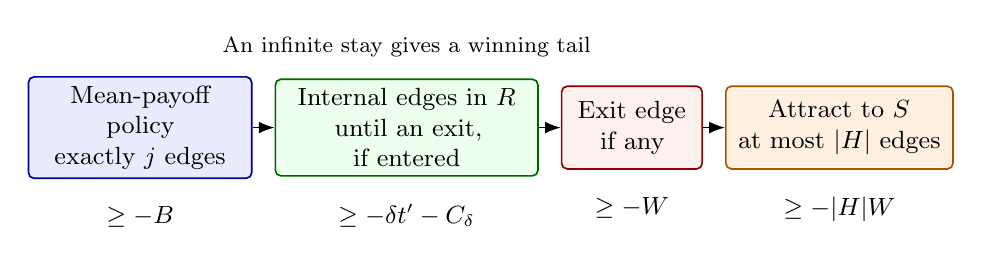
\begin{tikzpicture}[>=Latex,font=\small,
 block/.style={draw,rounded corners=2pt,minimum height=1.05cm,align=center},
 every path/.style={line width=.6pt}]
 \node[block,fill=blue!8,draw=blue!60!black,text width=2.6cm] (mp)
   {Mean-payoff policy\\exactly $j$ edges};
 \node[block,fill=green!7,draw=green!40!black,text width=3.1cm,
   right=.28cm of mp] (res)
   {Internal edges in $R$\\until an exit, if entered};
 \node[block,fill=red!6,draw=red!55!black,text width=1.55cm,
   right=.28cm of res] (exit)
   {Exit edge\\if any};
 \node[block,fill=orange!12,draw=orange!65!black,text width=2.65cm,
   right=.28cm of exit] (attr)
   {Attract to $S$\\at most $|H|$ edges};
 \draw[->] (mp)--(res);
 \draw[->] (res)--(exit);
 \draw[->] (exit)--(attr);
 \node[below=.22cm of mp,align=center] {$\ge-B$};
 \node[below=.22cm of res,align=center] {$\ge-\delta t'-C_\delta$};
 \node[below=.22cm of exit,align=center] {$\ge-W$};
 \node[below=.22cm of attr,align=center] {$\ge-|H|W$};
 \node[above=.15cm of res,align=center,font=\footnotesize]
   {An infinite stay gives a winning tail};
\end{tikzpicture}
\caption{A round in the even-priority construction of
Lemma~\ref{lem:combine}, with lower bounds for the weights of finite
prefixes of its parts. The $R$-part and its exit edge are omitted when the mean-payoff
part ends in $A$. Block widths are schematic. Every completed round
$j$ uses at least $j$ edges, which bounds the number of completed rounds
by time $T$ by $O(\sqrt T)$.}
\label{fig:round}
\end{figure}


\subsection{Determinacy with uniform prefix bounds}

We next establish that the strategies required on $R$ in the combination
lemma are always available at the winning vertices of \Max.  Proving
this assertion jointly with determinacy avoids any assumption that an
arbitrary winning strategy already has uniform prefix bounds.
The induction follows the attractor reduction in
\cite[Algorithm~3 and Appendix~C]{ChatterjeeHenzingerSvozil2017},
carrying the quantitative property through each removal.

\begin{theorem}
\label{thm:determinacy}
In every finite arena, each vertex is winning for exactly one of \Max\
and \Min.  From each vertex winning for \Max, there is a
conjunction-winning strategy satisfying \eqref{eq:uniform-prefix}.
\end{theorem}

\begin{proof}
We prove both assertions by induction on the number of vertices.  They
are vacuous in the empty arena.  Let $H$ be nonempty and assume the
assertions for all smaller arenas.

First observe how a nonempty set of already established winners reduces
the induction.  Suppose $Y\subseteq H$ is nonempty and every vertex of
$Y$ is winning for a player $J$, with strategies satisfying
\eqref{eq:uniform-prefix} if $J=\Max$.  Every vertex of
$Z=\Attr_J^H(Y)$ is also winning for $J$: attract to $Y$, then start a
winning strategy from the vertex reached.  Attraction lasts at most
$|H|$ edges.  If $J=\Max$, its bounded loss and the finite choice of
target strategies preserve \eqref{eq:uniform-prefix}.

Apply the induction hypothesis to the smaller arena $H\setminus Z$.
It is closed at $J$'s vertices.  A strategy there for the opponent of
$J$ can therefore keep play in this subarena and remains winning in
$H$.  A strategy there for $J$ is followed until any exit to $Z$, at
which point $J$ starts the winning strategy in $H$ associated with the
entry vertex.  There is at most one such switch: the new strategy is
continued on all subsequent histories, even if it later leaves $Z$.
Prefix independence proves that this strategy wins.

When $J=\Max$, the switch also preserves the quantitative property.
For each $\epsilon>0$, the internal prefix in $H\setminus Z$ and the
prefix after the switch have lower bounds of the form
$-\epsilon t_1-C_1$ and $-\epsilon t_2-C_2$.  The intervening edge costs
at most $W$, where $W$ bounds the absolute weights in $H$.  Taking the
constants in common over the finitely many possible entry vertices
gives a bound with slope $-\epsilon$ and constant $C_1+C_2+W$.
Prefixes before a switch satisfy the first bound.  If $J=\Min$, the
winning strategies of \Max\ remain entirely in the subarena and retain
their prefix bounds without switching.  Thus finding such a nonempty
$Y$ proves both assertions for $H$.

Let $d=\min_{v\in H}p(v)$, let $P$ be \Max\ for even $d$ and \Min\
for odd $d$, and let $Q$ be the other player.  Set
\[
 S=\{v\in H:p(v)=d\},\qquad
 A=\Attr_P^H(S),\qquad R=H\setminus A.
\]
If $d$ is even and \Max\ does not win for mean payoff alone everywhere
in $H$, Proposition~\ref{prop:mp-interface} supplies a nonempty set of
vertices from which \Min\ can force failure of the mean-payoff
condition.  These are conjunction-losing vertices, so they provide
$Y$ with $J=\Min$ in the preceding reduction.  We may therefore assume
that the mean-payoff hypothesis of Lemma~\ref{lem:combine} holds whenever
$d$ is even.

Since $S$ is nonempty, $R$ has fewer vertices than $H$.  Apply induction
to the game on $R$.  If its $Q$-winning set is nonempty, these strategies
remain winning in $H$: $R$ is closed at $P$'s vertices, so $Q$ can keep
play there.  Their prefix bounds also remain valid when $Q=\Max$.
They provide the required set $Y$ with $J=Q$.

In the remaining case, $P$ wins everywhere in $R$, with the uniform
prefix property when $P=\Max$.  Lemma~\ref{lem:combine} now proves the
assertions for all of $H$.  Finally, a vertex cannot be winning for both
players, since their objectives are complementary.
\end{proof}

\subsection{A dominion outside the least-priority attractor}

We can now turn the combination lemma around.  If an opponent dominion
had no opponent-winning part outside the relevant attractor, the lemma
would give the other player a winning strategy throughout that dominion.
For parity games this is the extraction principle of
\cite[Lemma~2.3]{LehtinenParysScheweWojtczak2022}; here the even case
also requires the ordinary mean-payoff hypothesis.

\begin{lemma}[Dominion extraction]
\label{lem:extract}
Let $H$ be a nonempty arena and $d\geq0$ an integer such that
$p(v)\geq d$ for all $v\in H$.  Let $P=\Max$ if $d$ is even and
$P=\Min$ if $d$ is odd, and let $Q$ be the other player.  Put
\[
 S=\{v\in H:p(v)=d\},\qquad
 R=H\setminus\Attr_P^H(S).
\]
If $d$ is even, assume that \Max\ wins for mean payoff alone everywhere
in $H$.  Then every nonempty $Q$-dominion $D$ in $H$ contains a nonempty
$Q$-dominion of the game on $R$.  The conclusion allows
$S=\varnothing$.
\end{lemma}

\begin{proof}
Inside the induced game on $D$, form
\[
  R_D=D\setminus\Attr_P^D(D\cap S).
\]
Because $D$ is a $Q$-dominion, it is closed at $P$'s vertices in $H$.
The attractor complement $R_D$ is closed at $P$'s vertices in $D$, hence
also in $H$.  It is disjoint from $S$, so the attractor-avoidance
observation in Section~\ref{sec:arenas} gives $R_D\subseteq R$.

If $d$ is even, \Max\ wins for mean payoff alone everywhere in $D$ as
well.  Indeed, the choices of \Max\ under a winning strategy in $H$ remain
available in $D$, because $D$ is closed at \Max's vertices; \Min\ is
restricted to choosing edges in $D$.

Suppose that the game on $R_D$ has no $Q$-winning vertex.
Theorem~\ref{thm:determinacy} makes every vertex there winning for $P$,
with the uniform prefix property if $P=\Max$.  Apply
Lemma~\ref{lem:combine} to the arena $D$, using the target $D\cap S$
and its residual arena $R_D$.  All its hypotheses have just been
verified, so $P$ wins everywhere in $D$, contrary to the fact that $D$
is a nonempty $Q$-dominion.  This argument includes $R_D=\varnothing$,
when its winning-strategy hypothesis is vacuous.

Consequently the $Q$-winning set in $R_D$ is nonempty.  It is a
$Q$-dominion there, and it lifts to a $Q$-dominion in $R$ by
Lemma~\ref{lem:arena-facts}, since $R_D$ is closed at $P$'s vertices.
It is contained in $D$, as required.  If $S=\varnothing$, then
$R=H$ and $R_D=D$; the same argument applies.
\end{proof}

\section{Recursion with bounded-dominion guarantees}
\label{sec:algorithm}

The structural results of the preceding section let us adapt the
reduced-precision recursion for parity games of Parys~\cite{Parys2019}.
The recursive output is a partition into two labels.  At intermediate
calls, its guarantee concerns only dominions below prescribed size
bounds.  Keeping this distinction explicit is essential: a vertex
labelled for a player need not yet be a winning vertex for that player.

\providecommand{\Solve}{\operatorname{Solve}}
\providecommand{\Phase}{\operatorname{Phase}}
Let $n$ be the number of vertices of the original arena.  For a subarena
$H$ and a pair of integer bounds
$\mathbf b=(b_{\Max},b_{\Min})\in\{0,\ldots,n\}^2$, the procedure
$\Solve(H,\mathbf b)$ returns a partition
$(\Lambda_{\Max},\Lambda_{\Min})$ of $H$.  We will prove that, for each
$J\in\{\Max,\Min\}$,
\begin{equation}
\label{eq:label-guarantee}
 D\text{ is a $J$-dominion in $H$ and }|D|\le b_J
 \quad\Longrightarrow\quad D\subseteq\Lambda_J.
\end{equation}
The call with both bounds equal to $n$ will therefore identify the
winning regions exactly.  Smaller bounds allow the recursion to make
most of its calls with one bound halved.

\subsection{The procedure}

There are three immediate cases.  If $H=\varnothing$, return two empty
sets.  If $b_{\Max}=0$, label every vertex $\Min$; this convention also
covers the case in which both bounds are zero.  If $b_{\Max}>0$ and
$b_{\Min}=0$, label every vertex $\Max$.

In all remaining cases, define
\[
 d=\min_{v\in H}p(v),\qquad
 P=\begin{cases}\Max,&d\text{ even},\\ \Min,&d\text{ odd},\end{cases}
 \qquad Q\ne P,
\]
where $Q$ is the other player.  Write
\[
 b=b_Q,\qquad b'=\lfloor b/2\rfloor,
 \qquad b^-_P=b_P,\quad b^-_Q=b',
\]
so that $\mathbf b^-$ is obtained from $\mathbf b$ by halving the
$Q$-bound.  The values $d,P,Q,\mathbf b,\mathbf b^-$ remain fixed until
this call returns.  The arena $U$, initially equal to $H$, changes by
deletions.  For each of its current values put
\begin{equation}
\label{eq:current-residual}
 S_U=\{v\in U:p(v)=d\},\qquad
 R_U=U\setminus\Attr_P^U(S_U).
\end{equation}
In particular, $R_U=U$ if $S_U=\varnothing$.

The subroutine of Proposition~\ref{prop:mp-interface} computes
$U_{\mathrm{mp}}(U)$, the ordinary mean-payoff winning set of $\Max$
in $U$.  We next define a local procedure $\Phase(U)$, which uses the
fixed parameters of its enclosing call and returns a subset of its
input arena.

\begin{quote}
\textbf{Procedure $\Phase(U)$.}
While $U\ne\varnothing$, perform the following steps.
\begin{enumerate}
\item If $d$ is even, compute $X=U\setminus U_{\mathrm{mp}}(U)$.
      If $X\ne\varnothing$, replace
      $U$ by $U\setminus\Attr_Q^U(X)$ and restart the while loop.
\item Form $R_U$ using~\eqref{eq:current-residual}.  Call
      $\Solve(R_U,\mathbf b^-)$, and let $C$ be its $Q$-labelled set.
      If $C=\varnothing$, return the current $U$.
\item Replace $U$ by $U\setminus\Attr_Q^U(C)$ and restart the while loop.
\end{enumerate}
If the while loop ends because $U=\varnothing$, return $\varnothing$.
\end{quote}

The enclosing call uses two reduced phases separated by a single call
with unchanged bounds. The first phase rules out small $Q$-dominions
in $R_U$. If a $Q$-dominion of size at most $b$ still survives in $U$,
Lemma~\ref{lem:extract} consequently supplies more than $b'$ of its
vertices in a $Q$-dominion of $R_U$. The intervening unchanged-bounds
call deletes those vertices. At most $b'$ vertices of the original
dominion then remain, which is why one final reduced phase suffices.

\noindent\begin{minipage}{\linewidth}
The precise procedure for $\Solve(H,\mathbf b)$ is:
\begin{enumerate}
\renewcommand{\labelenumi}{\textnormal{(\roman{enumi})}}
\item Set $U=H$, and then replace $U$ by $\Phase(U)$.
\item If $U\ne\varnothing$, form $R_U$ and make the single call
      $\Solve(R_U,\mathbf b)$ with both bounds unchanged.  Let $C$ be its
      $Q$-labelled set, and replace $U$ by
      $U\setminus\Attr_Q^U(C)$.
\item Replace $U$ by $\Phase(U)$ once more.
\item Return $\Lambda_P=U$ and $\Lambda_Q=H\setminus U$.
\end{enumerate}
\end{minipage}\par\medskip
Calling the phase on the empty arena has no effect.  Every deletion is
an attractor deletion, so every restriction used here is an arena by
the attractor-complement property in Section~\ref{sec:arenas}.

We now prove the claimed removal of $Q$-dominions together with the
preservation of $P$-dominions.

\subsection{Termination and correctness}

\begin{theorem}[Bounded-dominion guarantee]
\label{thm:labels}
For every subarena $H$ of the original game and every
$\mathbf b\in\{0,\ldots,n\}^2$, the procedure
$\Solve(H,\mathbf b)$ terminates and returns a partition satisfying
\eqref{eq:label-guarantee} for both players.
\end{theorem}

\begin{proof}
We induct on the number of distinct priorities in $H$.  The empty-arena
and zero-bound cases terminate immediately and have the stated
guarantee: the only dominion subject to a zero size bound is empty, and
the other player receives the whole arena.

Consider a call with $H\ne\varnothing$ and both bounds positive.  Its
fixed value $d$ occurs in $H$.  Every child arena $R_U$ excludes all
vertices of priority $d$ and is a subset of $H$.  It therefore has
strictly fewer distinct priorities than $H$, so the induction hypothesis
applies to every child.  This remains true if $d$ has disappeared from
$U$ before the child is formed: the strict decrease is relative to the
parent's input $H$, even when $R_U=U$.  Each continuation of a phase loop
deletes a nonempty set.  Thus its children terminate by induction, its
loop can continue at most $|H|$ times, and the enclosing call terminates.

\emph{Preservation of $P$-dominions.}
Fix a $P$-dominion $D$ in $H$ with $|D|\le b_P$.  We show that every
deletion leaves all of $D$ in the current arena and preserves it there
as a $P$-dominion.  Suppose this holds immediately before a deletion.
For a deletion in the mean-payoff step, $P=\Max$.  A winning strategy
that stays in $D$ also wins for mean payoff alone in $U$, so
$D\cap X=\varnothing$.  Since $D$ is closed at $Q$'s vertices,
Lemma~\ref{lem:arena-facts} shows that
$\Attr_Q^U(X)$ misses $D$ and preserves its dominion property in the
residual arena.

For a deletion obtained from a recursive call, the restriction $R_U$
is closed at $P$'s vertices.  The same lemma therefore makes
$D\cap R_U$ a $P$-dominion in $R_U$.  Its size is at most $b_P$, and
both kinds of child call retain this bound for $P$.  By the induction
hypothesis, the child labels every vertex of $D\cap R_U$ for $P$.
Its $Q$-labelled set $C\subseteq R_U$ is consequently disjoint from
$D$.  Again $\Attr_Q^U(C)$ misses $D$ and preserves it as a dominion.
This argument applies to deletions in either phase and in the
unchanged-bounds stage.  Hence $D$ lies in the returned set $\Lambda_P$.
In particular, this reasoning uses only the child's guarantee on small
dominions; it does not require that every vertex of $C$ actually be
winning for $Q$.

\emph{Removal of $Q$-dominions.}
Fix a $Q$-dominion $D$ in $H$ with $|D|\le b$.  Every current arena is
obtained from the preceding one by removing a $Q$-attractor.  Each such
restriction is closed at $Q$'s vertices.  Applying the intersection
part of Lemma~\ref{lem:arena-facts} after each deletion gives
\begin{equation}
\label{eq:surviving-q-dominion}
 D\cap U\text{ is a $Q$-dominion in the current arena }U.
\end{equation}
Unlike the preceding preservation argument, this assertion allows some
vertices of $D$ to have been deleted.

Suppose a phase returns a nonempty arena $U$.  It did so because its
last reduced-bound child returned no $Q$-labelled vertices.  The
induction hypothesis then implies that
\begin{equation}
\label{eq:phase-end}
 R_U\text{ contains no nonempty $Q$-dominion of size at most }b'.
\end{equation}
Moreover, when $d$ is even, the mean-payoff step immediately before
that child certified $U_{\mathrm{mp}}(U)=U$.  Thus, at a nonempty phase
return, all hypotheses of Lemma~\ref{lem:extract} hold in $U$: every priority
is at least $d$, and the required mean-payoff condition holds when $d$
is even.  No occurrence of priority $d$ in the current $U$ is required.

Let $U_1$ be the arena returned by the first phase.  If $D\cap U_1$
is nonempty, it is a $Q$-dominion there by
\eqref{eq:surviving-q-dominion}.  Lemma~\ref{lem:extract} gives a
nonempty $Q$-dominion $E$ of the game on $R_{U_1}$ such that
\[
 E\subseteq D\cap U_1,\qquad b'<|E|\le b.
\]
Here the strict lower bound follows from~\eqref{eq:phase-end}.
The unchanged-bounds child has $Q$-bound $b$, so it labels all of $E$
for $Q$.  Its subsequent attractor deletion therefore removes at least
$b'+1$ vertices of $D$, leaving at most
$|D|-(b'+1)\le b-b'-1\le b'$ vertices.  If $D\cap U_1$ was
already empty, no vertices of $D$ remain.  Thus, in either case, the
arena $U$ at the start of the final phase satisfies
\begin{equation}
\label{eq:half-remainder}
 |D\cap U|\le b'.
\end{equation}

Let $U_2$ be the arena returned by the final phase.  If $D\cap U_2$
were nonempty, it would be a $Q$-dominion in $U_2$ of size at most $b'$
by~\eqref{eq:surviving-q-dominion} and~\eqref{eq:half-remainder}.
Applying Lemma~\ref{lem:extract} once more would produce a nonempty
$Q$-dominion in $R_{U_2}$ of size at most $b'$, contradicting
\eqref{eq:phase-end}.  Therefore $D\cap U_2=\varnothing$, and every
vertex of $D$ receives label $Q$.  The two arguments prove the
induction step for both players.
\end{proof}

To solve the original arena $G$, call $\Solve(G,(n,n))$ and return its
$\Max$-labelled set.  By Theorem~\ref{thm:determinacy}, the two winning
regions partition $G$, and the winning-region observation in
Section~\ref{sec:arenas} makes each a dominion.  Their sizes are at most
$n$, so Theorem~\ref{thm:labels} labels both regions correctly.  It remains to
bound the cost of computing this partition.

\section{Complexity in the full binary input length}
\label{sec:complexity}

We first bound the recursion independently of the cost of solving an
ordinary mean-payoff game.  This separates the combinatorial reduction
from the numerical subroutine and shows exactly where the full binary
encoding enters the running time.

\begin{proposition}[Cost of the reduction]
\label{prop:reduction-cost}
For an arena with $n\ge1$ vertices and complete binary input length $L$,
the call $\Solve(G,(n,n))$ makes
\[
 2^{O((\log_2(n+2))^2)}
\]
calls to the ordinary mean-payoff winning-set subroutine.  Each such
call has an explicit input of length $(L+2)^{O(1)}$.  Apart from those
subroutine calls, the computation takes
\[
 2^{O((\log_2(n+2))^2)}(L+2)^{O(1)}
\]
bit operations.  All constants are absolute.
\end{proposition}

\begin{proof}
Consider the tree of calls to $\Solve$, counting its immediate base
cases as nodes.  Every child omits the minimum priority of its parent's
input arena.  Thus a path has at most $n$ edges, independently of the
numerical values of the priorities.

Each node has at most one child with both size bounds unchanged.
Every other child has one bound halved, with rounding down.  In either
phase, a child is followed by a nonempty deletion unless that phase
returns.  Each phase therefore makes at most $n+1$ child calls, giving
at most
\[
 M=2(n+1)
\]
children with a halved bound at a node.  Along a path, either one of the
two size bounds can be halved at most $1+\lfloor\log_2 n\rfloor$
times before reaching zero, where the recursion stops.  Consequently,
there are at most
\[
 h=2(1+\lfloor\log_2 n\rfloor)
\]
halving edges on any path.

The resulting path count is the same combinatorial saving that
underlies reduced-precision parity recursion~\cite{Parys2019}.
For a path of length $\ell$ with $j$ halving edges, choose their
positions and, at each one, the child index among at most $M$ halving
children.  At every remaining position there is at most one available
unchanged-bounds child.  This gives at most $\binom{\ell}{j}M^j$ paths
of that type.  As each node is specified by its root-to-node path, the
total number of calls $N_{\rm rec}$ satisfies
\begin{align}
\label{eq:recursion-count}
 N_{\rm rec}
 &\le \sum_{\ell=0}^{n}\sum_{j=0}^{\min(\ell,h)}
          \binom{\ell}{j}M^j\\
 &\le (n+1)(h+1)(nM)^h
  =2^{O((\log_2(n+2))^2)}.\nonumber
\end{align}
The second inequality uses $\binom{\ell}{j}\le n^j$ and $nM\ge1$;
it also covers $n=1$.

We next count the nonrecursive work at a node.  A phase iteration that
continues deletes at least one vertex.  The two phases together
therefore make at most $n+2$ iterations, allowing one final return
iteration for each phase.  In particular, they make $O(n+1)$ ordinary
mean-payoff calls.  Attractor computations, construction of induced
subarenas, scans for minimum priorities, and updates of the two size
bounds all take polynomially many bit operations in $L+2$.  No step
iterates through the integers between two successive priority values:
minimum priorities and equality tests are computed directly from their
binary encodings.

All mean-payoff instances use induced subarenas of the original graph,
with the weights $w(v,u)=r(v)$.  Renumbering retained vertices uses only
polynomial space and time.  Even if the reward $r(v)$ is copied
explicitly onto every retained outgoing edge, the total number of
weight bits is at most the number of edges times the largest original
reward bit length, hence polynomial in $L+2$.  The rest of each
subroutine input is also polynomial in $L+2$.  This proves the claimed
input-length bound without a dependence on the numerical magnitude
of a reward.  Combining these per-node bounds with
\eqref{eq:recursion-count} proves the proposition.
\end{proof}

\begin{proof}[Proof of Theorem~\ref{thm:main}]
The empty arena has an empty winning set and is handled immediately.
For a nonempty arena, the output of $\Solve(G,(n,n))$ is exact by
Theorem~\ref{thm:labels} and the winning-region argument at the end of
Section~\ref{sec:algorithm}.

Proposition~\ref{prop:mp-interface} implements each ordinary mean-payoff
call of input length $L'$ in
$2^{O((\log_2(L'+2))^2)}$ bit operations, uniformly and deterministically.
By Proposition~\ref{prop:reduction-cost}, there is an absolute constant
$a$ such that $L'\le(L+2)^a$ for every call, after increasing $a$ if
necessary.  Its cost is therefore
$2^{O((\log_2(L+2))^2)}$.  The number of calls and all remaining work
have the same bound, since $n$ is polynomially bounded by the explicit
input length.  Their product is again
\[
 2^{O((\log_2(L+2))^2)}.
\]
All graph operations and recursion choices admit deterministic
implementations, so the complete procedure has the stated uniform
deterministic bit complexity.  In particular, the constants do not
depend on the number of priorities or on the numerical sizes of the
binary rewards and priorities.
\end{proof}

\bibliographystyle{plain}
\bibliography{references}
\end{document}
